\subsubsection{Scopo}
Include le attività e i compiti svolti per creare il \gl{prodotto}.
\subsubsection{Aspettative}
Le aspettative della corretta implementazione del processo sono:
\begin{itemize}
		\item realizzare un prodotto finale conforme alle richieste del \gl{proponente} e che soddisfi le attività di \gl{validazione} e \gl{verifica};
		\item fissare gli obiettivi di sviluppo;
		\item fissare i vincoli tecnologici.
\end{itemize}

\subsubsection{Descrizione}
In accordo con lo standard \iso{ISO/IEC 12207}, il processo di sviluppo è composto dalle attività di:
\begin{itemize}
		\item analisi dei requisiti;
		\item progettazione;
		\item codifica;
		\item validazione.
\end{itemize}

\subsubsection{Analisi dei requisiti}
 \paragraph{Scopo dell'attività}
  Individuare i requisiti del \gl{progetto} dalle specifiche del \gl{capitolato} e tramite incontri con il pro-
  ponente. Tale attività produrrà un documento redatto dagli analisti, i quali avranno cura di elencare i \gl{casi d'uso} e i requisiti. Tale documento permette di
 capire le scelte di progettazione effettuate.
 \paragraph{Aspettative dell'attività}
 L'attività fissa come scopo la creazione di un documento che elencherà e rappresenterà i requisiti richiesti dal proponente.
 \paragraph{Descrizione dell'attività}
 Tutti i requisiti analizzati, utilizzando le specifiche del capitolato e consultando i proponenti negli
incontri effettuati, vanno specificati nell'\ARdoc. Per analizzare e trovare i
requisiti si utilizza la tecnica dei casi d'uso. Il tracciamento dei requisiti avviene tramite l'applicativo PragmaDB.

 \paragraph{Casi d'uso}
 Ogni caso d'uso è così composto:
 \begin{itemize}
  \item \textbf{Codice identificativo}: codice univoco del caso d'uso in esame;
  \item \textbf{Titolo}: indica il titolo del caso d'uso;
  \item \textbf{Diagramma \gl{UML}}: rappresenta graficamente il caso d'uso;
  \item \textbf{Attori primari}: indica gli attori primari coinvolti;
  \item \textbf{Descrizione}: chiara, precisa e concisa descrizione del caso d'uso;
  \item \textbf{Precondizione}: indica la situazione che deve essere vera prima dell'esecuzione del caso d'uso;
  \item \textbf{Postcondizione} indica la situazione che deve essere vera dopo l'esecuzione del caso d'uso;
  \item \textbf{Scenario principale}: descrizione composta dal flusso dei casi d'uso figli;
  \item \textbf{Scenari alternativi}: descrizione composta dai casi d'uso che non appartengono al flusso
principale di esecuzione.
 \end{itemize}
 \paragraph{Codice identificativo dei casi d'uso}
Ogni caso d'uso ha un proprio codice identificativo  che rispetta il seguente formalismo:\\ \\
\centerline{UC\textbraceleft{Codice}\textbraceright{}}
\\ \\dove:
\begin{itemize}
	\item \textbf{Codice}: indica il codice identificativo del requisito, è univoco e deve essere identificato in forma gerarchica.
\end{itemize}
 \paragraph{Requisiti}
 Ogni requisito è così composto:
  \begin{itemize}
  \item \textbf{Codice identificativo}: codice univoco del requisito;
  \item \textbf{Descrizione}: una breve descrizione, deve essere meno ambigua possibile;
  \item \textbf{Fonti}: identifica la fonte dalla quale è stato identificato il requisito.
 \end{itemize}
 \paragraph{Codice identificativo dei requisiti}
 Ogni requisito individuato avrà un codice identificativo univoco così formato: \\ \\
 \centerline{R\textbraceleft{}Tipo\textbraceright{}\textbraceleft{}Importanza\textbraceright{}\textbraceleft{}Codice\textbraceright{}}
 \\ \\
 dove:
 \begin{itemize}
 	\item \textbf{Tipo}: può assumere uno di questi valori:
 	\begin{itemize}
 		\item \textbf{F}: indica un requisito funzionale;
 		\item \textbf{Q}: indica un requisito di qualità;
 		\item \textbf{P}: indica un requisito prestazionale;
 		\item \textbf{V}: indica un requisito di vincolo.
 	\end{itemize}
 	\item \textbf{Importanza}: può assumere uno di questi valori:
 	\begin{itemize}
 		\item \textbf{O}: indica un requisito obbligatorio;
 		\item \textbf{D}: indica un requisito desiderabile;
 		\item \textbf{F}: indica un requisito facoltativo.
 	\end{itemize}
 	\item \textbf{Codice}: indica il codice identificativo del requisito, è univoco e deve essere identificato in forma gerarchica.
 \end{itemize}
 \paragraph{UML}
 Viene utilizzata la versione corrente alla stesura del documento, ovvero la 2.5.
 \subsubsection{Progettazione}\label{progettazione}
 \paragraph{Scopo dell'attività}
 L'attività di progettazione definisce le linee essenziali della struttura del prodotto \gl{software} in
 funzione dei requisiti individuati dall'analisi. L'obiettivo del processo consiste nella stesura dei
 documenti: \textit{"Specifica Tecnica"} e \textit{"Definizione di \gl{Prodotto}"}. \\
 Compresi pienamente quali siano i requisiti del problema e approfondendo la progettazione a moduli
 abbastanza semplici da essere capiti da una sola persona, si otterranno le
 istruzioni necessarie ai \PRP{} per sviluppare il prodotto.\\
 La progettazione deve utilizzare le seguenti tipologie di diagrammi UML:
 \begin{itemize}
 	\item \textbf{Diagrammi delle classi}: illustrano una collezione di elementi dichiarativi di un modello	come classi e tipi, assieme ai loro contenuti e alle loro relazioni;
 	\item \textbf{Diagrammi dei \gl{packages}}: raggruppamenti di classi in una unità di livello più alto;
 	\item \textbf{Diagrammi di attività}: illustrano il flusso di operazioni relativo ad un’attività; utilizzati	soprattutto per descrivere la logica di un algoritmo. Nel contesto del progetto \PROGETTO, questo tipo di diagramma potrebbe rappresentare bene il flusso del dialogo con l'assistente virtuale;
 	\item \textbf{Diagrammi di sequenza}: descrivono una determinata sequenza di azioni dove tutte le
 	scelte sono già state effettuate; in pratica nel diagramma non compaiono scelte, né flussi
 	alternativi.
 \end{itemize}
 \paragraph{Aspettative dell'attività}
 Il processo porta alla formazione dei documenti sopracitati, i quali garantiscono affidabilità e
 coerenza.
 \paragraph{Descrizione dell'attività}
 La progettazione deve rispettare tutti i vincoli e i requisiti concordati tra i componenti del gruppo
 e i proponenti. I documenti derivati da questa attività sono:
 \begin{itemize}
 	\item \textbf{Specifica tecnica}: descrive la progettazione ad alto livello relativa all'architettura dell'applicazione
 	e dei singoli componenti. Il documento specifica i diagrammi UML ed i design
 	pattern utilizzati per realizzare l'architettura definendo inoltre i test necessari alla verifica;
 	\item \textbf{Definizione di prodotto}: descrive in dettaglio la progettazione di \gl{sistema}, integrando
 	quanto scritto nella Specifica Tecnica. Il documento specifica i diagrammi UML e le
 	definizioni delle classi definendo inoltre i test necessari alla verifica.
 \end{itemize}

 \paragraph{Requisiti per i progettisti}\label{req prog}
 I \PJP{} sono responsabili delle attività di progettazione. Essi sono tenuti ad avere:
 \begin{itemize}
 	\item profonda conoscenza di tutto ciò che riguarda il processo di sviluppo del software;
 	\item capacità di saper anticipare i cambiamenti;
 	\item notevole inventiva per riuscire a trovare una soluzione progettuale accettabile anche in
mancanza di una metodologia che sia sufficientemente espressiva;
 	\item capacità di individuare con rapidità e sicurezza le soluzioni più opportune.
 \end{itemize}

 \paragraph{Specifica tecnica}\label{Specifica tecnica}
 I \PJP{} devono definire la struttura ad alto livello dell'architettura del sistema e dei singoli
componenti, raccogliendo il tutto nella \textit{"Specifica Tecnica"}. Devono, inoltre, essere definiti i test di
integrazione tra le varie componenti, che verranno inseriti in appendice al Piano di Qualifica.
I prodotti di questo \gl{task} saranno:
 \begin{itemize}
 	\item \textbf{Diagrammi UML}:
 	\begin{itemize}
 		\item diagrammi delle classi;
 		\item diagrammi dei package;
 		\item diagrammi di attività;
 		\item diagrammi di sequenza.
 	\end{itemize}
 	\item \textbf{\gl{Design pattern}}: devono essere descritti i design pattern utilizzati per realizzare l'architettura. Ogni design
 	pattern deve essere accompagnato da una descrizione ed un diagramma, che ne esponga il
 	significato e la struttura;
 	\item \textbf{Tracciamento delle componenti}: ogni componente dovrà essere tracciato ed associato
 	ad almeno un requisito. In tal modo sarà possibile avere la certezza che tutti i requisiti
 	accettati siano soddisfatti e che ogni componente presente nell’architettura soddisfi almeno
 	un requisito. Tale tracciamento dovrà essere effettuato tramite PragmaDB, che si occupa
 	di generare in modo automatico le relative tabelle;
 	\item \textbf{Test di integrazione}: i \PJP{} devono definire delle strategie di verifica per poter dimostrare la corretta integrazione tra le varie componenti definite. Questi test dovranno poi essere inseriti nel \doc{Piano di Qualifica}.
 \end{itemize}
 \paragraph{Definizione di prodotto}\label{definizione prodotto}
 I \PJP, a partire dalla \textit{"Specifica Tecnica"}, devono produrre la \textit{"Definizione di Prodotto"} dove
viene descritta la progettazione di dettaglio del sistema. Lo scopo di questo documento è quello di
definire dettagliatamente ogni singola unità di cui è composto il sistema in modo da semplificare
l'attività di codifica e allo stesso tempo di non fornire alcun grado di libertà al \PR.
Parallelamente alla progettazione di dettaglio dei componenti software dovranno essere progettati
i relativi test di unità che verranno descritti nel  \textit{"Piano di Qualifica"}. I prodotti di questo task
saranno:
 \begin{itemize}
 	\item \textbf{Diagrammi UML}:
 	\begin{itemize}
 		\item diagrammi delle classi;
 		\item diagrammi di attività;
 		\item diagrammi di sequenza.
 	\end{itemize}
 	\item \textbf{Definizioni delle classi}: ogni classe progettata deve essere descritta in modo da spiegarne lo scopo e definirne le
 	funzionalità ad essa associate. Per ogni classe dovranno essere anche definiti i vari metodi e attributi che la caratterizzano;
 	\item \textbf{Tracciamento delle classi}: ogni classe deve essere tracciata ed associata ad almeno un requisito, in questo modo è possibile avere la certezza che tutti i requisiti accettati siano	soddisfatti e che ogni classe presente nell’architettura soddisfi almeno un requisito. Questo 	tracciamento dev’essere effettuato tramite PragmaDB, che si occupa di generare in modo automatico le tabelle di tracciamento;
 	\item \textbf{Test di unità}: i \PJP{} devono definire le strategie di verifica delle varie classi in modo che durante l’attività di codifica sia possibile verificare che la classe si comporti in modo corretto. Questi test dovranno poi essere inseriti nel \doc{Piano di Qualifica}.
 \end{itemize}
 \paragraph{Stile di progettazione}
 Con lo scopo di aumentare la manutenibilità del sistema, i progettisti devono seguire
 le seguenti regole:
 \begin{itemize}
 	\item la progettazione deve essere corretta rispetto lo standard UML versione 2.5;
 	\item l’architettura non deve presentare problemi di progettazione che possano compromettere la qualità del sistema;
 	\item ogni libreria esterna deve essere rappresentata come un package di colore arancione, differente quindi dalle componenti interne progettate;
 	\item gli attributi di una classe possono essere pubblici solo se essa non definisce nè un costruttore nè alcun metodo per impostarne i valori;
 	\item i metodi di una classe possono essere privati solo se sono di supporto ad uno o più metodi pubblici. Un metodo privato può comunque essere di supporto ad un altro metodo privato;
 	\item i nomi dei package e delle classi devono essere autoesplicativi e in lingua inglese;
 	\item qualora ci si riferisca ad un attributo, metodo, classe o componente, il suo nome deve essere contenuto all'interno del comando \file{\textbackslash file\{\}}. Inoltre, il nome dovrà essere preceduto dal suo scoping nel caso l'oggetto sia di una classe o componente esterne rispetto a quella soggetta.
 \end{itemize}
 \subparagraph{Modularizzazione delle componenti}
 I \PJP{} dovranno definire e adottare delle tecniche di modularizzazione affinchè l’architettura software progettata sia di elevata qualità, permettendo così la scomposizione del sistema in moduli. Inoltre, è necessario fornire una descrizione precisa della struttura modulare e delle relazioni che esistono tra i singoli moduli.

 \subsubsection{Codifica}
 \paragraph{Scopo dell'attività}
 Lo scopo dell'attività è l'implementazione del prodotto, concretizzando la soluzione tramite la codifica.
 \paragraph{Aspettative dell'attività}
 L'aspettativa dell'attività è un prodotto corretto, ovvero stabile, affidabile, funzionale e che soddisfi i requisiti.
 \paragraph{Descrizione dell'attività}
 L'attività deve rispettare i compiti e gli strumenti espressi nel \PPdoc.
 \paragraph{Stile}

 Al fine di rendere il codice più leggibile possibile, il gruppo dovrà rispettare le seguenti regole:
 \begin{itemize}
 	\item il codice deve essere identato al meglio, in particolare se uno o più statement sono interni a una porzione di codice, essi dovranno rientrare di due spazi (come suggeriscono Google, npm, \gl{Node.js}, Idiomatic, Felix), come nell'esempio che segue: \begin{lstlisting}
 	if(condition)
 	{
 	  a=b;
 	  b=c;
 	}
 	\end{lstlisting}
 	\item le parentesi graffe che vanno a delimitare un blocco di codice dovranno trovarsi al di sotto della sua segnatura, come negli esempi che seguono:
 	\begin{lstlisting}
 	while(condition)
 	{
 	  operazioni
 	}

 	void foo()
 	{
	  operazioni
 	}
 	\end{lstlisting}
 	\item le costanti devono essere scritte in maiuscolo;
 	\item le variabili devono rispettare le seguenti regole:
 	\begin{itemize}
 		\item avere un nome più esplicativo possibile;
 		\item se il nome è composto da più parole, esse devono essere divise da un carattere di underscore ' \textbf{\_} ';
 		\item essere composti da una singola lettera, come i o j, esclusivamente per gli indici a ciclo breve;
 		\item essere, se possibile, inizializzate ad un valore.
 	\end{itemize}
 	\item i metodi e funzioni devono rispettare le seguenti regole:
 	\begin{itemize}
 		\item avere un nome più esplicativo possibile;
 		\item se composto da più parole, il nome deve seguire la notazione camelCase;
 		\item evitare un numero eccessivo di parametri.
 	\end{itemize}
 	\item evitare l'eccessivo innestarsi di statement.
 \end{itemize}
In caso di codice seguente il paradigma della programmazione asincrona, devono essere seguite anche le seguenti regole:
\begin{itemize}
	\item le funzioni di \gl{callback} dovranno essere scritte in una solo linea esclusivamente se contengono una sola istruzione. In tal caso, dovranno essere scritte secondo la notazione a freccia (arrow function) descritta in ECMAScript 2015;\\
	 In caso contrario, si dovranno seguire le regole precedentemente esposte;
	 \item l'annidamento di funzioni di callback deve essere evitato e sostituito seguendo il costrutto delle Promise descritto in ECMAScript 2015.
\end{itemize}

I seguenti esempi vogliono essere dei chiarimenti delle regole appena descritte.
\begin{lstlisting}
collection_one . forEach (( item ) => { console . log ( item )});
collection_two . forEach ( function ( item )
{
  item = Math . random ();
  console .log( item );
});
\end{lstlisting}


\paragraph{Documentazione del codice}\label{intestazione}
Per facilitare la manutenibilità del codice, i programmatori devono rispettare le seguenti norme sulla documentazione:
\begin{itemize}
 \item ogni file dovrà avere un'intestazione formata nel seguente modo:
 \begin{lstlisting}
 /**
 * Descrizione della classe.
 * @author Autore
 * @version Versione corrente del file o della classe
 * @since Versione del prodotto nel quale e' presente il file o la classe
 */
 \end{lstlisting}
 \item ogni metodo di una classe dovrà contenere un'intestazione formata nel modo seguente:
 \begin{lstlisting}
 /**
 * Breve descrizione del metodo.
 * @param {tipo_Parametro1} NomeParametro1 Descrizione del primo parametro
 * ...
 * @param {tipo_ParametroN} NomeParametroN Descrizione del N-esimo parametro
 * @return {tipo_ritorno} breve descrizione di cosa il metodo ritorna, se diverso da null.
 */

 \end{lstlisting}
 \item scrivere dei commenti in italiano qualora certe porzioni di codice possano risultare poco chiare o complesse;
 \item evitare di commentare porzioni di codice dal funzionamento banale;
 \item aggiungere commenti al codice costituito da cicli e diramazioni logiche. Si tratta di aree
 	di fondamentale importanza che facilitano la lettura del codice sorgente;
 \item separare i commenti dai delimitatori di commento con spazi vuoti. In questo modo i
 	commenti saranno chiari e facili da individuare.
\end{itemize}
 \paragraph{Ricorsione}
 La \gl{ricorsione} va evitata. Se non risulta accettabile convertirla in \gl{iterazione}, bisogna fornirne la prova di terminazione e l'analisi del costo in termini di spazio.

 \paragraph{Fogli di stile}
 Per la produzione di fogli di stile viene usato \textbf{Sass}, un linguaggio di scripting interpretato in CSS. In particolare vengono usati files con estensione \textit{.scss}, che consiste in un ampliamento del linguaggio CSS.

\paragraph{Regole JavaScript}
La parte del prodotto codificata in JavaScript deve seguire le seguenti regole:
\begin{itemize}
	\item gli operatori == e != effettuano conversioni di tipo prima di effettuare il confronto, e ciò potrebbe nascondere errori di tipo. È meglio utilizzare gli operatori === e !== in quanto meno propensi a \textit{side-effects};
	\item il metodo alert() non dovrebbe mai essere utilizzato, in quanto comporta problemi di usabilità e sicurezza;
	\item in un ciclo for il contatore deve operare sulla stessa variabile della condizione di loop;\\
Esempio di codice non valido:
\begin{verbatim}
  for (i = 0; i < 10; j++)  // Variabili diverse, codice non valido
  {
    // ...
  }
\end{verbatim}
	\item lo statement for..in permette lo scorrimento di tutti i nomi delle proprietà di un certo oggetto. Vengono però incluse anche tutte le proprietà ereditate dai prototipi, rendendo quindi necessaria la presenza di un filtro all'interno del ciclo.\\
Esempio di codice non valido:
\begin{verbatim}
  for (name in object)
  {
    doSomething(name);
  }
\end{verbatim}
Esempio di codice valido:
\begin{verbatim}
  for (name in object)
  {
    if (object.hasOwnProperty(name))
    {
      doSomething(name);
    }
  }
\end{verbatim}
	\item NaN non deve essere usato per fare qualunque tipo di confronto;
	\item l'utilizzo dell'operatore new deve avvenire solo con oggetti che possiedono una funzione che ha il ruolo di costruttore;
	\item lo statement switch deve contenere default come clausola finale. Questo serve per evitare situazioni anomale;
	\item in un ciclo for il contatore deve muoversi nella direzione giusta, al fine di evitare cicli infiniti. Se l'obiettivo è la creazione di un ciclo infinito, è meglio utilizzare altri statement, come il while.\\
Esempio di codice non valido:
\begin{verbatim}
  for (var i = 0; i < strings.length; i--)
  {
    //...
  }
\end{verbatim}
	\item L'unione di una serie di if annidati comporta maggiore comprensibilità del codice.\\
Esempio di codice non valido:
\begin{verbatim}
  if (x !== undefined)
  {
    if (x === 2)
    {
      // ...
    }
  }
\end{verbatim}
Esempio di codice valido:
\begin{verbatim}
  if (x !== undefined && x === 2)
  {
    // ...
  }
\end{verbatim}
	\item evitare la presenza di statement vuoti. Nel caso in cui siano necessari, bisogna giustificarne la presenza con un commento atto a spiegare il ruolo dello statement;

	\item la modifica dei contatori di loop all'interno di un ciclo è rischiosa perchè può portare a cicli infiniti, e di conseguenza va evitata. Se si vuole far fronte a particolari situazioni all'interno di un ciclo è preferibile l'utilizzo di una variabile flag;

	\item le variabili devono essere dichiarate prima di essere usate, al fine di stabilirne lo scoping, usando var se sono variabili con scope globale, let se sono variabili locali e const se sono variabili da non modificare;
	\item ogni statement deve terminare con ";", al fine di aumentare la comprensibilità del codice.

\end{itemize}

\paragraph{Continuous integration}\label{CI}
I programmatori devono caricare il codice sorgente nel repository pubblico \url{https://github.com/CoCodeSWE/AtAVi}.
Ogni commit deve recare un messaggio che spieghi concisamente le aggiunte o le modifiche che sono state apportate al codice. Gli amministratori hanno configurato un sistema di integrazione continua con Jenkins, in modo che ogni commit scateni
una build del codice esistente e l'esecuzione di tutti i test di unità, integrazione e sistema. \\
Nel caso in cui si verifichi un errore, il programmatore che ha effettuato il commit verrà notificato attraverso una mail e dovrà correggere al più presto i problemi del codice.

 \subsubsection{Procedure}
 \paragraph{Inserimento di un attore in PragmaDB}
 Per inserire un attore in PragmaDB è necessario applicare la seguente procedura:
 \begin{itemize}
 	\item effettuare l'accesso in PragmaDB;
 	\item selezionare la voce "Attori";
 	\item selezionare la voce "Inserisci Attore";
 	\item inserire nome e descrizione dell'attore.
 \end{itemize}
 \paragraph{Inserimento di un caso d'uso in PragmaDB}
 Per inserire un caso d'uso in PragmaDB è necessario applicare la seguente procedura:
 \begin{itemize}
 	\item effettuare l'accesso in PragmaDB;
 	\item selezionare la voce "Use Case";
 	\item selezionare la voce "Inserisci Use Case";
 	\item popolare tutti i campi richiesti;
 	\item inserire gli attori coinvolti;
 	\item inserire i requisiti correlati.
 \end{itemize}
 \paragraph{Inserimento di una fonte in PragmaDB}
 Per inserire una fonte in PragmaDB è necessario applicare la seguente procedura:
 \begin{itemize}
 	\item effettuare l'accesso in PragmaDB;
 	\item selezionare la voce "Fonti";
 	\item selezionare la voce "Inserisci Fonte";
 	\item inserire nome e descrizione della fonte.
 \end{itemize}
 \paragraph{Inserimento di un requisito in PragmaDB}
 Per inserire un requisito in PragmaDB è necessario applicare la seguente procedura:
 \begin{itemize}
 	\item effettuare l'accesso in PragmaDB;
 	\item selezionare la voce "Requisiti";
 	\item selezionare la voce "Inserisci Requisito";
 	\item popolare tutti i campi richiesti;
 	\item inserire la fonte correlata;
 	\item inserire l'use case correlato.
 \end{itemize}
 \paragraph{Inserimento di un package in PragmaDB}
 Per inserire un package in PragmaDB è necessario applicare la seguente procedura:
 \begin{itemize}
 	\item effettuare l'accesso in PragmaDB;
 	\item selezionare la voce "\gl{Package}";
 	\item selezionare la voce "Inserisci Package";
 	\item popolare tutti i campi richiesti.
 \end{itemize}
 \paragraph{Inserimento di una classe in PragmaDB}
 Per inserire una classe in PragmaDB è necessario applicare la seguente procedura:
 \begin{itemize}
 	\item effettuare l'accesso in PragmaDB;
 	\item selezionare la voce "Classi";
 	\item selezionare la voce "Inserisci Classe";
 	\item popolare i campi richiesti;
 	\item inserire i requisiti correlati.
 \end{itemize}
 \paragraph{Tracciamento requisiti-fonti}
 Per tracciare una fonte su un requisito è sufficiente, al momento della creazione del requisito, inserire la fonte correlata. Se questo non è stato fatto, è necessario applicare la seguente procedura:
 \begin{itemize}
 	\item effettuare l'accesso in PragmaDB;
 	\item selezionare la voce "Requisiti";
 	\item selezionare la voce "Modifica" del requisito interessato;
 	\item selezionare e inserire la fonte correlata.
 \end{itemize}
 \paragraph{Tracciamento classi-requisiti}
 Per tracciare un requisito su una classe è sufficiente, al momento della creazione della classe, inserire il requisito correlato. Se questo non è stato fatto, è necessario applicare la seguente procedura:
 \begin{itemize}
 	\item effettuare l'accesso in PragmaDB;
 	\item selezionare la voce "Classe";
 	\item selezionare la voce "Modifica" della classe interessata;
 	\item selezionare e inserire il requisito correlato.
 \end{itemize}
 \paragraph{Tracciamento package-requisiti}
 Per realizzare questo tracciamento è sufficiente applicare il tracciamento classi-requisiti, in quanto il relativo package contenitore è dedotto automaticamente da PragmaDB.
 \paragraph{Produzione automatica del documento \DPdoc}
 Il documento \DPdoc{} è generato automaticamente da PragmaDB, il quale produrrà il relativo codice \LaTeX{} da compilare.
 Per far ciò, è necessario seguire la seguente procedura:
 \begin{itemize}
 	\item effettuare l'accesso in PragmaDB;
 	\item selezionare la voce "Classi";
 	\item selezionare le voci:
 	\begin{itemize}
 		\item "Genera Classi";
 		\item "Tracciamento Classi-Requisiti";
 		\item "Tracciamento Requisiti-Classi";
 		\item "Tracciamento Componenti-Requisiti";
 		\item "Tracciamento Requisiti-Componenti";
 		\item "Genera immagini";
 		\item "Segnali";
 	\end{itemize}
 	\item selezionare la voce "Homepage";
 	\item selezionare la voce "Package";
 	\item selezionare le voci:
 	\begin{itemize}
 		\item "Genera Package";
 		\item "Tracciamento Componenti-Requisiti";
 		\item "Tracciamento Requisiti-Componenti";
 	\end{itemize}
 	\item aprire il file \DPfile;
 	\item in quest'ultimo file includere i file .tex generati da pragmaDB con il comando \begin{lstlisting}
 	input{nomeFile}
 	\end{lstlisting}
 	seguendo questo ordine:
 	\begin{itemize}
 		\item package;
 		\item classi;
 		\item tracciamentoClassiRequisiti;
 		\item tracciamentoRequisitiClassi;
 		\item tracciamentoClassiComponenti;
 		\item tracciamentoComponentiClassi;
 		\item tracciamentoComponentiRequisiti;
 		\item tracciamentoRequisitiComponenti.
 	\end{itemize}
 \end{itemize}
 Sarà cura dei \PJP{} produrre e posizionare i diagrammi di sequenza.
\paragraph{Produzione automatica del documento \ARdoc}
Il documento \ARdoc{} è generato automaticamente da PragmaDB, il quale produrrà il relativo codice \LaTeX{} da compilare.
Per far ciò, è necessario seguire la seguente procedura:
\begin{itemize}
	\item effettuare l'accesso in PragmaDB;
	\item selezionare la voce "Use Case";
	\item selezionare tutte le voci sotto "Esporta in \LaTeX";
	\item tornare nella home page;
	\item selezionare la voce "Requisiti";
	\item selezionare tutte le voci sotto "Esporta in \LaTeX";
	\item aprire il file \ARfile;
	\item in quest'ultimo file includere i file .tex generati da pragmaDB con il comando \begin{lstlisting}
	input{nomeFile}
	\end{lstlisting}
	seguendo questo ordine:
	\begin{itemize}
		\item useCase;
		\item requisiti;
		\item tracciamentoFontiRequisiti;
		\item tracciamentoRequisitiFonti;
		\item riepilogoRequisiti;
	\end{itemize}
\end{itemize}

\subsubsection{Strumenti}
 \paragraph{PragmaDB}
  PragmaDB è uno strumento \gl{open source} di tracciamento dei requisiti. Verrà quindi utilizzato per semplificare e automatizzare il più possibile l'attività di analisi dei requisiti e di progettazione. In particolare, una volta inseriti casi d'uso, attori, requisiti, fonti, classi e package, PragmaDB genera:
  \begin{itemize}
  \item il codice \LaTeX{} relativo a casi d'uso e requisiti in forma tabellare;
  \item i diagrammi UML associati ai casi d'uso;
  \item il diagramma UML di ogni classe.

  \end{itemize}
  Essendo open source, questo strumento è stato adattato dal \gl{team} \GRUPPO{} in base alle proprie necessità.
  \paragraph{Astah}
  Astah è uno strumento di modellazione UML. Qualora i diagrammi UML generati da PragmaDB non siano soddisfacenti, si ricorrerà all'utilizzo di Astah. Viene utilizzata la versione 7.0 o superiori.
\begin{figure}[h]
\centering
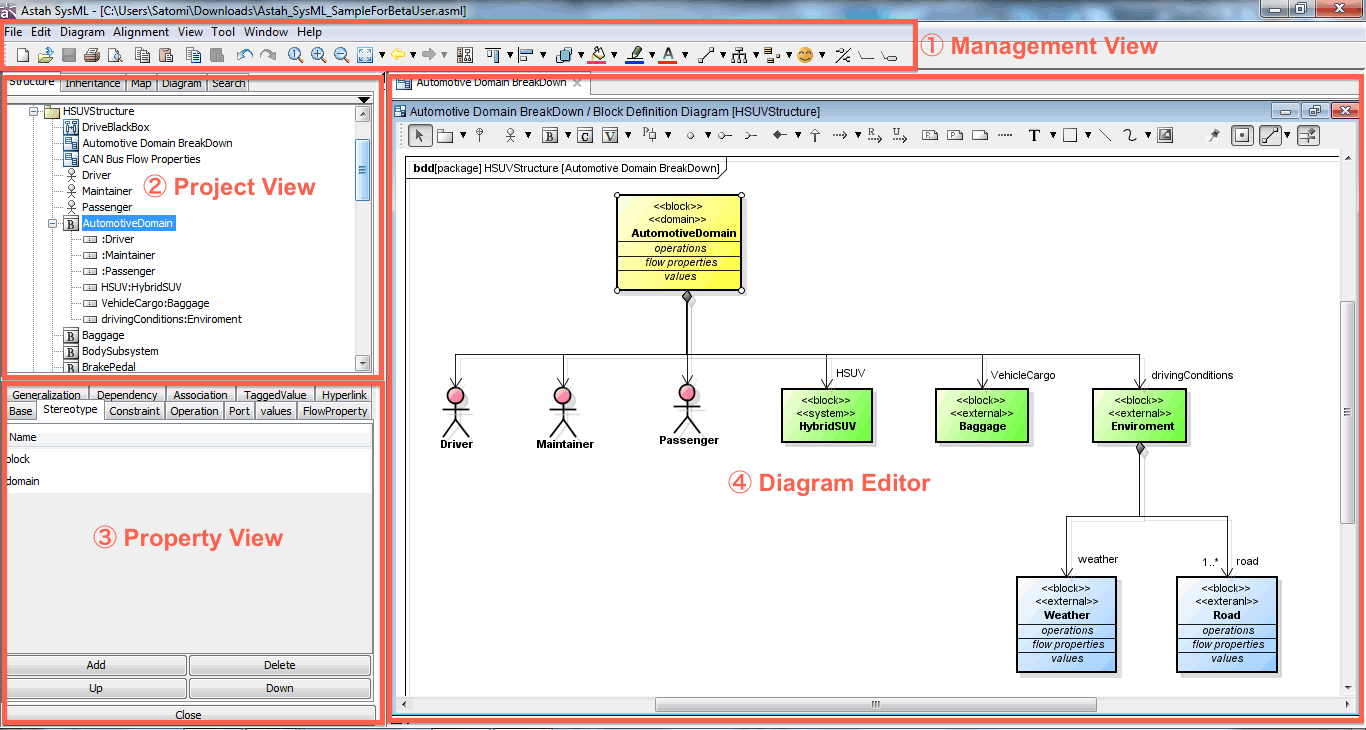
\includegraphics[scale=0.3]{img/astah.png}
\caption{Astah}\label{sec:Figura1}
\end{figure}

\paragraph{Atom}
Il gruppo ha deciso di utilizzare Atom come IDE per scrivere il codice sorgente. Questo strumento offre molte funzionalità utili, tra le quali l'integrazione diretta con \gl{Git} oltre ad essere cross-platform.

\paragraph{api.ai}
api.ai è lo strumento che verrà adottato per lo sviluppo dell'assistente virtuale, per gestire le interazione con gli utenti del sistema.
\begin{figure}[h]
\centering
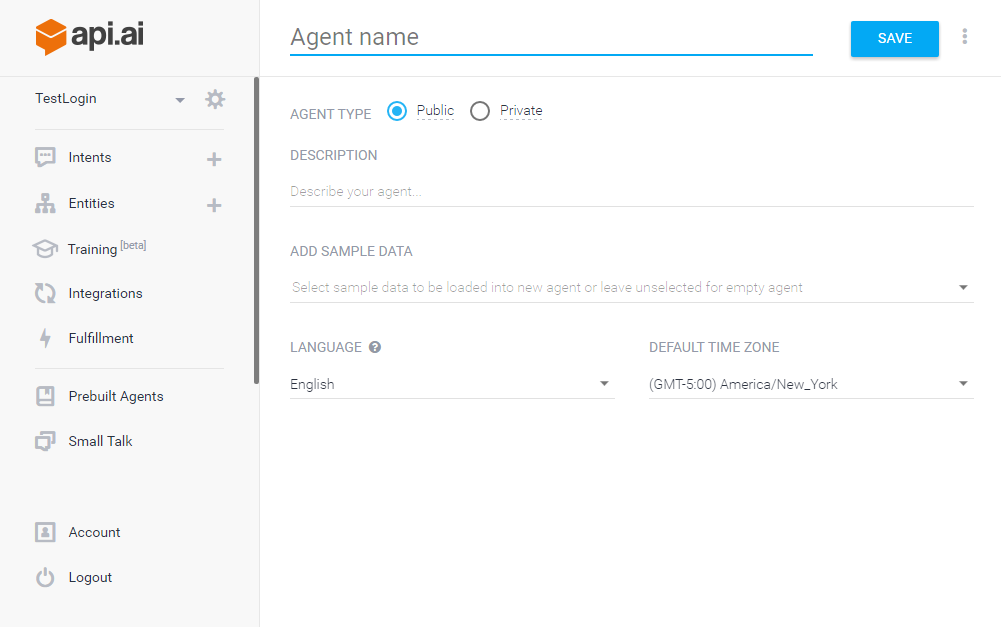
\includegraphics[scale=0.5]{img/api_ai.png}
\caption{api.ai}\label{sec:Figura1}
\end{figure}

\newpage
